\documentclass{article}
\usepackage[utf8]{inputenc}

\title{Support Vector Machines}
\author{Sylesh Suresh}
\date{October 2017}

\usepackage{natbib}
\usepackage{graphicx}
\usepackage{bm}
\usepackage{listings}
\usepackage{mathtools}          %loads amsmath as well
\usepackage{tikz}
\usepackage{pgfplots}

\begin{document}

\maketitle

\section{Introduction}
Support Vector Machines (SVMs) are one of the most popular supervised learning models today, able to perform both linear and nonlinear classification.
\section{Linear Classification}
The idea behind SVMs is to maximize the margin, the distance between the hyperplane (decision boundary) and the samples nearest to this hyperplane, called support vectors. 
\begin{figure}[h!]
\centering
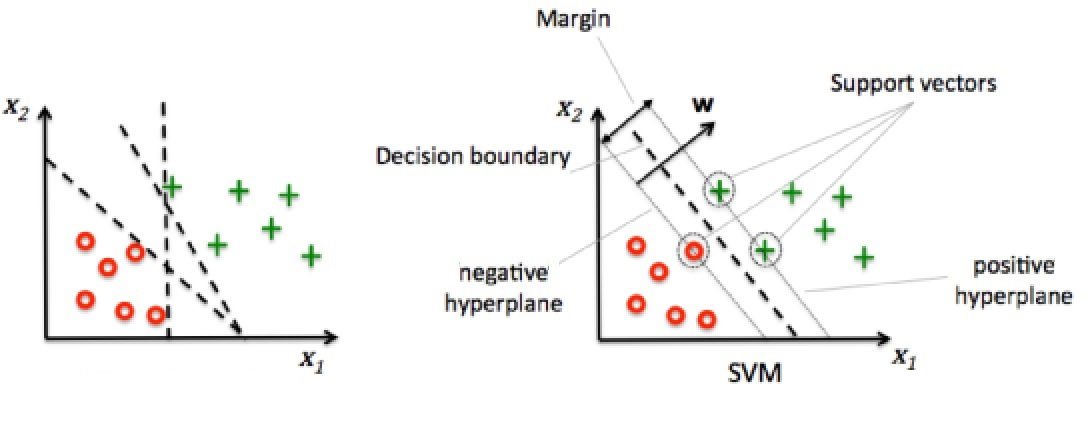
\includegraphics[scale=0.4]{svm.jpg}
\caption{Support Vector Machine}
\label{fig:svm}
\end{figure}
The decision boundaries to the left separate the training data correctly but would not generalize well to unseen data, being too close to the training samples (i.e. having a small margin). On the other hand, the decision boundary to the right marked by the dashed line separates the training data and generalizes well to unseen data, having a large margin. Maximization of the margin allows for the least generalization error.

$\bm{w}$ is defined as a vector normal to the decision boundary. 
The positive hyperplane is defined as
\[ \bm{w \cdot x_{pos}} + w_0 = 1 \]
while the negative hyperplane is:
\[ \bm{w \cdot x_{neg}} + w_0 = -1 \]

We can combine these equations by subtracting the second equation from the first:
\begin{equation} \label{eq:hyperplanes}
\bm{w}{(x_{pos} - x_{neg})} = 2 
\end{equation}

To calculate the margin, first, let us take the difference between a positive support vector and a negative support vector.

\[ x_{pos} - x_{neg} \]

Then, we need to multiply this by a unit vector perpendicular to the hyperplanes. We earlier defined $\bm{w}$ to be normal to the hyperplanes, so $\frac{\bm{w}}{||\bm{w}||}$ serves this purpose:

\[ \frac{\bm{w}(x_{pos} - x_{neg})}{||\bm{w}||} \]
Using ~\ref{eq:hyperplanes}, we arrive at:

\[ \frac{\bm{w}(x_{pos} - x_{neg})}{||\bm{w}||} = \frac{2}{||\bm{w}||} \]

We must maximize $\frac{2}{||\bm{w}||}$ to maximize the margin. For mathematical convenience, we can minimize $\frac{1}{2}{||\bm{w}||^2}$ to achieve the same effect. The constraint for this optimization problem is that the samples are actually classified correctly:

\[ \bm{w \cdot x_{i}} + w_0 = 1 \text{ if $y_i = 1$} \]

\[ \bm{w \cdot x_{i}} + w_0 = -1 \text{ if $y_i = -1$}\]
where $x_i$ is a particular sample and $y_i$ is the class of the sample. More compactly:

\[ y_i(w_0 + \bm{w \cdot x_i}) - 1 = 0 \]
Using Lagrange multipliers, we  calculate the following Lagrange function:

\[ L(\bm{w}, w_0) = \frac{1}{2}{||\bm{w}||^2} - \sum_i{a_i(y_i(w_0 + \bm{w \cdot x_i}) - 1)}\]
where $a_i$ is our Lagrange multiplier.

\[ \frac{\partial L}{\partial \bm{w}} = \bm{w} - \sum_i{{a_i}{\bm{x_i}}{y_i}} = 0\]
Thus, 
\[ \bm{w} = \sum_i{{a_i}{\bm{x_i}}{y_i}} \]

\[ \frac{\partial L}{\partial w_0} = -\sum_i{{a_i}{y_i}} = 0\]
Thus,
\[ \sum_i{{a_i}{y_i}} = 0 \]
Combining these equations finally yields
\[ L = \sum_i{a_i}  - \frac{1}{2}{\sum_i{\sum_j{{a_i}{a_j}{y_i}{y_j}{(\bm{x_i \cdot x_j})}}}} \]
which we can optimize through quadratic programming.

\section{Soft-Margin Classification}
Most of the time, our data will not be linearly separable. The standard method is to allow the SVM to misclassify some data points, and pay a cost for each misclassified point. We can accomplish this by adding a slack variable $\xi$. Our optimization problem becomes minimizing $\frac{1}{2}{||\bm{w}||^2} + C\sum_i{{{\xi}_i}}$ with the constraint $y_i(w_0 + \bm{w \cdot x_i}) \geq 1 - {\xi}_i$. $C$ is a regularization hyperparameter; if $C$ is set to be small, more misclassifications are allowed, but if $C$ is set to be large, less misclassifications are allowed. 

\section{Non-binary Classification}

SVM's are inherently useful for binary classification. However, they can also be used for data with more than two classes.

\subsection{One versus the Rest}
If we train an SVM to separated one class from all the other classes, and do this for each class, we can combine the SVMs for multi-class classification.
$$\mbox{argmax}\limits_{j=1 \dots M} g^j(x)$$

\[g^j(x) = \sum_{i=1}^{m}y_i a_{i}^j k(x, x_i) + b^j\]

\subsection{Pairwise Classification}
If we train an SVM for every possible combination of pairs of classes, we will train $\frac{n(n+1)}{2}$ SVMs for a dataset with $n$ classes. Classify a point by running it through all the SVMs and adding up the number of times the point is classified into each class. The class with the most number is considered the label.


\section{Nonlinear Classification using Kernels}
In the real world, data is usually not linearly separable, meaning that the support vector machine as cannot accurately separate the data. However, we can project the data onto a higher dimensional space where the data is linearly separable using a mapping function $\phi{(\cdot)}$ For example:
\[ \phi{(x_1, x_2)} = (z_1, z_2, z_3) = (x_1, x_2, x_1^2 + x_2^2) \]
Using this mapping function allows us to separate the two classes below (indicated by red and blue) with a linear hyperplane. We can then project this back into two-dimensional space where the decision boundary becomes nonlinear.

\begin{figure}[h!]
\centering
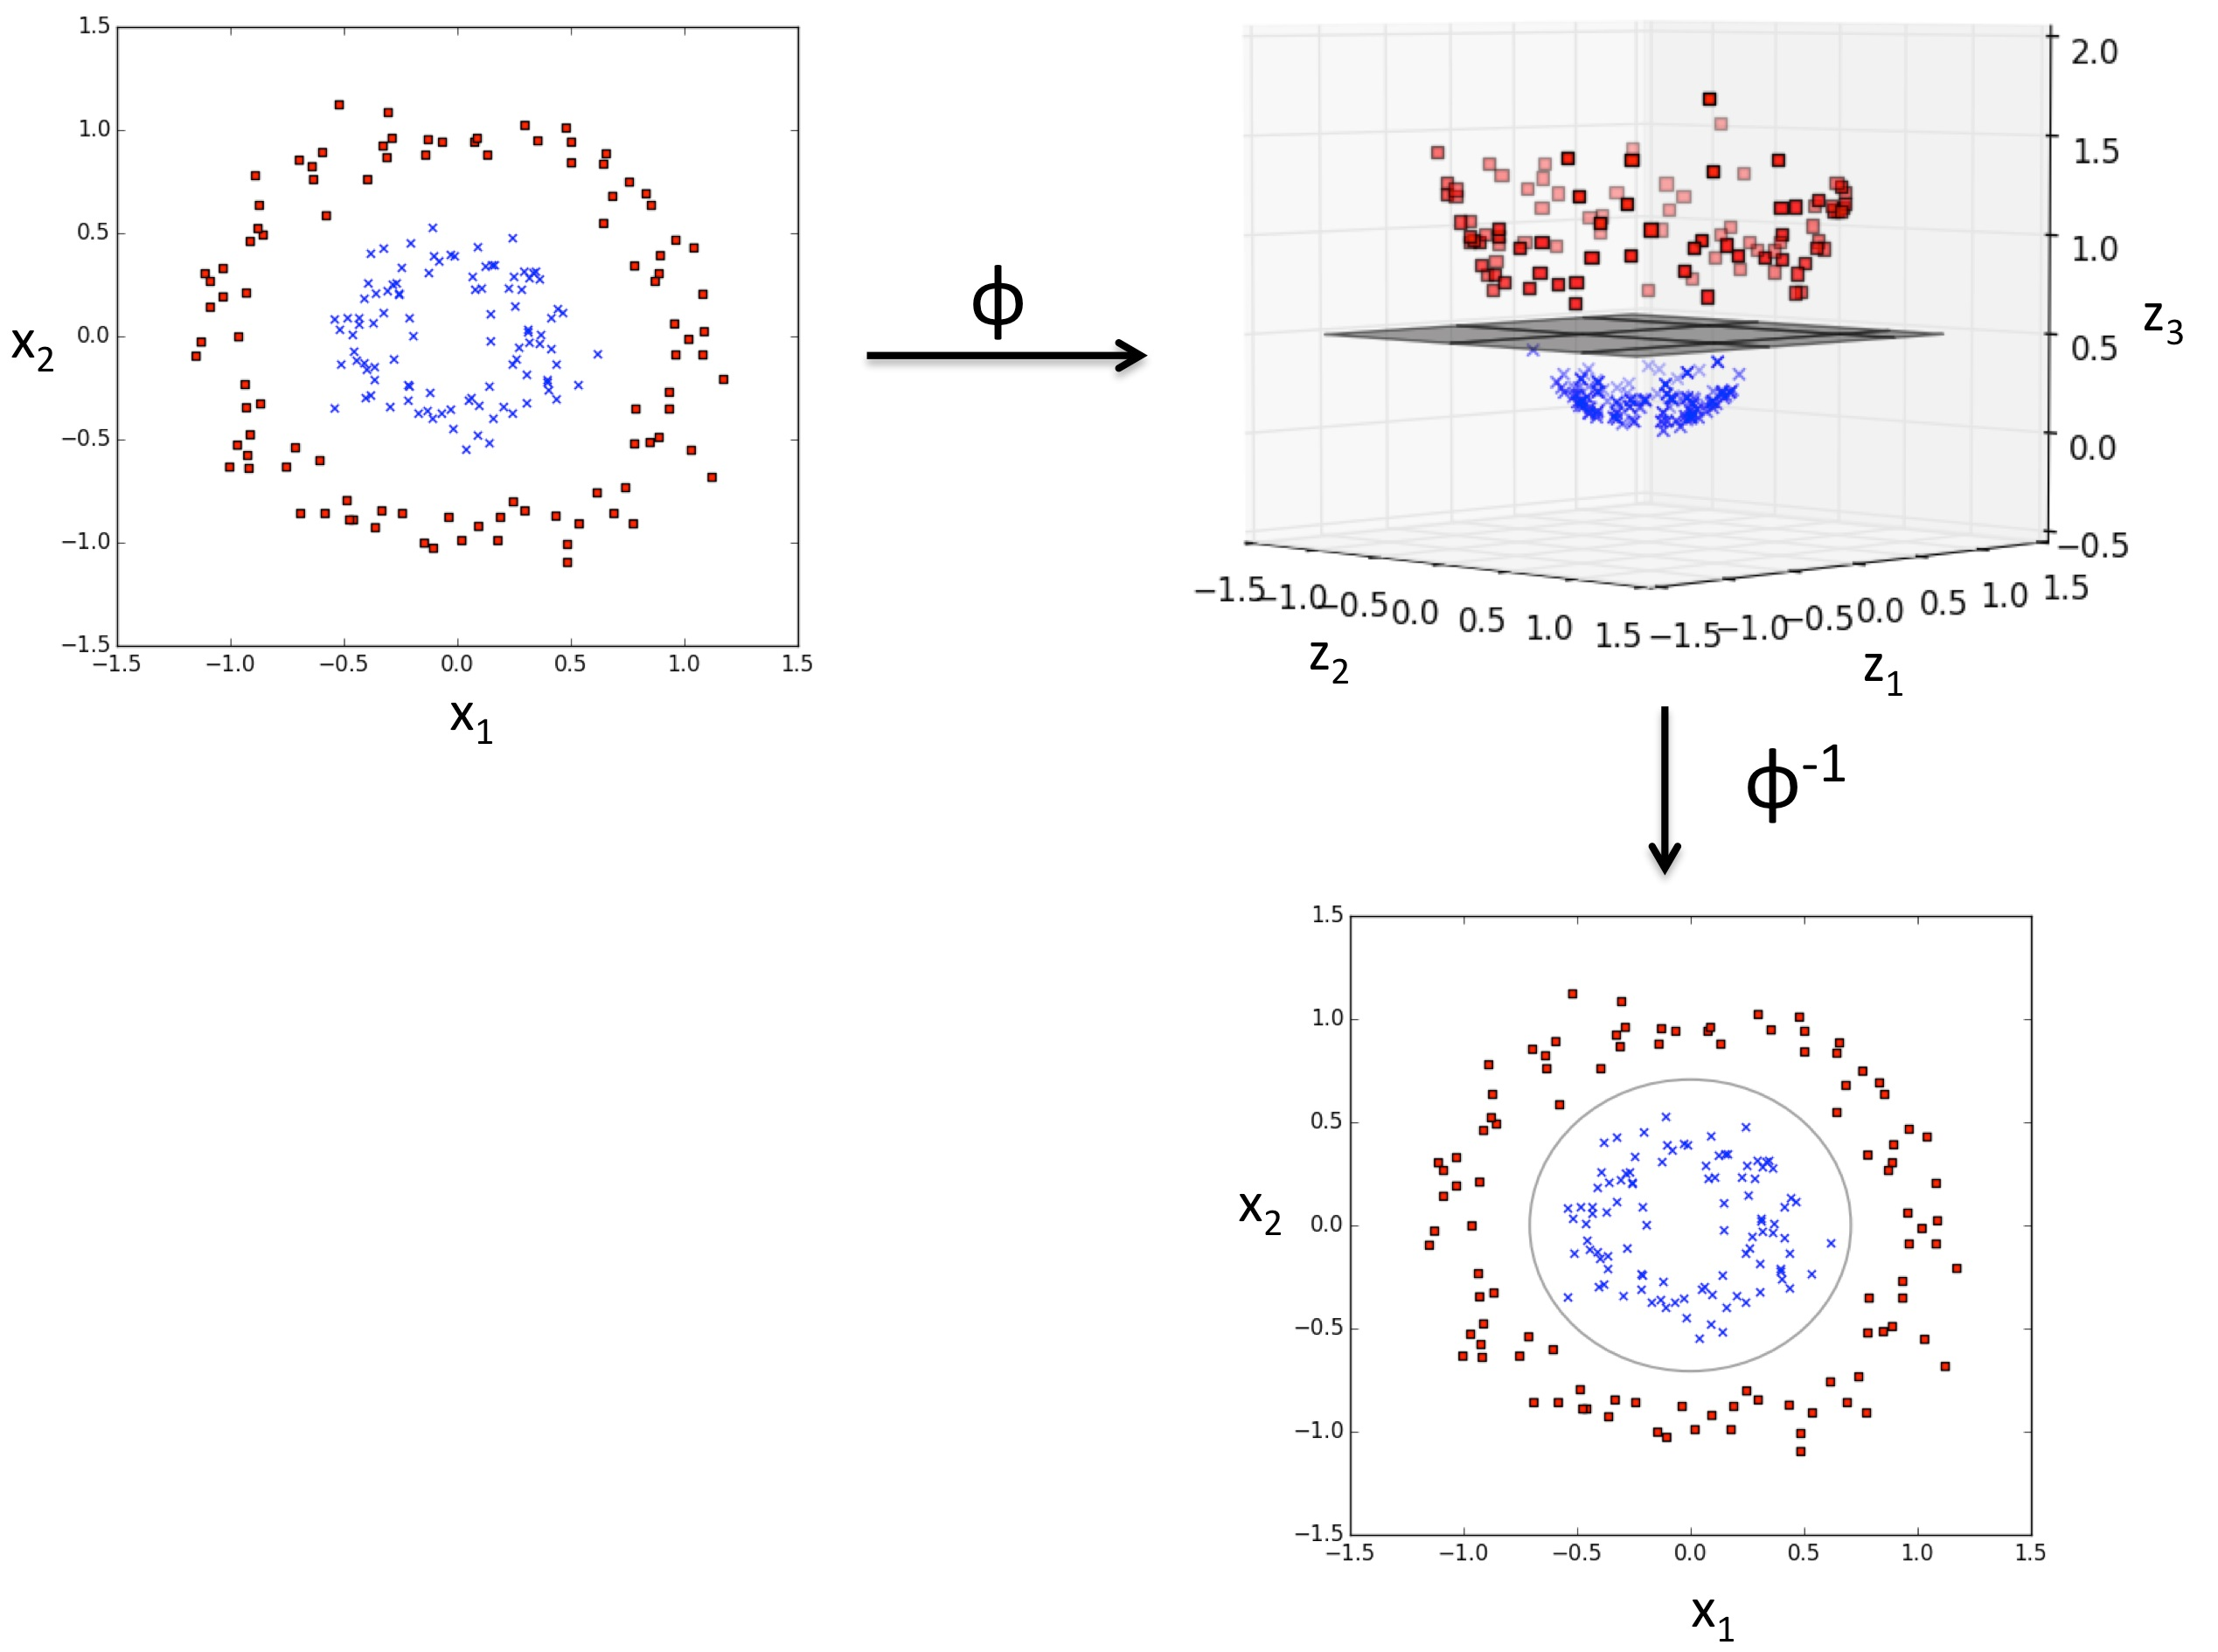
\includegraphics[scale=0.18]{dimensions.jpg}
\caption{Projecting to higher space}
\label{fig:mapping}
\end{figure}
The problem, however, with this approach is its efficiency. When solving the optimization problem of maximizing the margin, the pair-wise dot products of different training samples $\bm{x_i}$ and $\bm{x_j}$ must be calculated, a very computationally expensive process in high-dimensional space. To solve this, we can use the kernel trick; we can use kernel functions to implicitly calculate the dot product of $\bm{x_i}$ and $\bm{x_j}$ without explicitly projecting them into higher dimensional space. 

One of the most popular kernel functions is the Radial Basis Function kernel (RBF kernel) or Gaussian kernel:

\[ k(\bm{x_i}, \bm{x_j}) = \exp{(-\gamma||\bm{x_i}-\bm{x_j}||^2}) \]

$\gamma$ is a free parameter that can be optimized.

\section{Library}
To start off the year easy, we will be using Scikit-Learn, which has multi-class support built-in.

\lstinputlisting[language=Python, firstline=0, lastline=12]{svm.py}

\section{Practice Problem}
Given the following data:
\begin{center}
\begin{tabular}{ |c|c|c| } 
 \hline
 x1 & x2 & out \\
 \hline
 -1 & -2 & -1 \\ 
 -1 & 0 & -1 \\ 
 -3 & -5 & -1 \\ 
 2 & 0 & 1 \\ 
 3 & -2 & 1 \\
 0 & 1 & 1 \\
 
 \hline
\end{tabular}
\end{center}
Graphed on the following plane with the hyperplane $y + 2x =0$.
\begin{center}
\begin{tikzpicture}
\begin{axis}[
    axis lines=middle,
    xmin=-5, xmax=5,
    ymin=-5, ymax=5,
    xtick={-5,-4,-3,-2,-1,0,1,2,3,4,5}, ytick={-5,-4,-3,-2,-1,0,1,2,3,4,5}
]
\addplot [only marks] table {
-1 -2
-1 0
-3 -5
};
\addplot [only marks, mark=o] table {
2 0
3 -2
1 1
};
\addplot [domain=-10:10, samples=2, dashed] {-2*x};
\end{axis}
\end{tikzpicture}
\end{center}
\begin{enumerate}
\item Find the distance from the hyperplane to each of the points.
\item Find the margin of the hyperplane.
\end{enumerate}
\end{document}
